\scanpage{188}
Donc ces $\varphi$ correspondent exactement aux
\[
\xi_1\deleted{{}=A_1+B_1dX_0}\ \in\operatorname{Ker}\alpha=\mathcal A^+
\]
i.e. \deleted{\unsure{aux}} (posons $\xi_1=A_1+B_1dX_0$, $A_1,B_1\in\unsure{B|S}\{X_0\}$)
aux couples
\[
A_1\in S\{X_0\}^{+},\quad B_1\in S\{X_0\}
\]

\figure{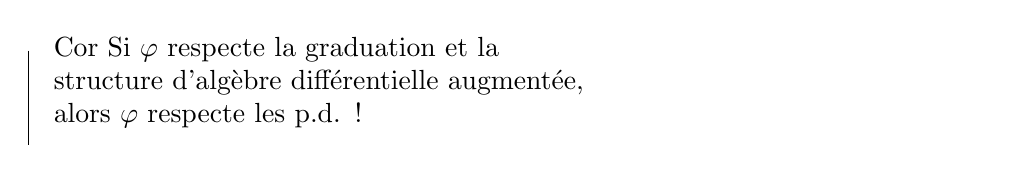
\begin{tikzpicture}
\draw (0,0)--(0,-1.2);
\node[anchor=north west,text width=12cm] at (.2,.3) {\uline{Cor} Si $\varphi$ respecte la graduation \uline{et} la\\
structure d'algèbre différentielle augmentée,\\
alors $\varphi$ respecte les p.d. !};
\end{tikzpicture}}

On prend maintenant $S=k\{T\}$, et
on regarde $S$ comme muni d'un idéal à
p.d. \deleted{\unsure{0}}\inserted{$k\{T\}^{+}$} pour $\mathcal A=\mathcal A_1$. Donc $\alpha$ est
compatible avec toutes ces structures, y
compris les p.d. On définit
\[
\begin{array}{rcll}
\beta:\mathcal A_1&=S\{X_0,dX_0\}=k\{T\}\{X_0,dX_0\}&\longrightarrow&S\\
&\simeq S\{X_0,X_1,dX_0,dX_1\}/(X_0+X_1-T,dX_0+dX_1)_{\mathrm{pd}}&&\text{\textquotedbl}\\
&&&k\{T\}
\end{array}
\]
par la condition que $\beta$ est comp. avec
toutes les structures, et
\margin{\figure{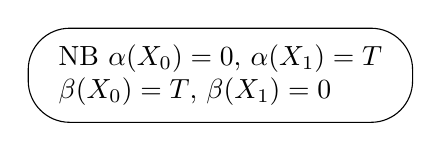
\begin{tikzpicture}
\node[draw,rounded corners=15pt,inner sep=5pt] {\begin{tabular}{ll}NB $\alpha(X_0)=0$, $\alpha(X_1)=T$\\
$\beta(X_0)=T$, $\beta(X_1)=0$\end{tabular}};
\end{tikzpicture}}}
\[
\beta(X_0)=T\qquad\text{donc}\quad
\begin{cases}\beta(X_0^{(i)})=T^{(i)}\\\beta(dX_0)=0\end{cases}
\]
et on s'intéresse aux $\varphi$ \inserted{(un hom. d'alg. diff. sur $S$)} compatibles
avec l'augmentation $\alpha$ \uline{et} $\beta$, Cela
signifie que l'on a $\beta\varphi=\beta$ i.e.
\[
\beta\underbrace{\varphi(X_0^{(i)})}_{A_1^{(i)}+B_i\,dX_0}
=\deleted{\unsure{\xi_1}}\beta(X_0^{(i)})\quad\text{pour }\forall i\geq1,\quad\text{ou encore}
\]
\[
\beta(A_1)^{(i)}=T^{(i)}\qquad\forall i\geq1\qquad\text{ou encore}
\]
\margin{187}
